% Standalone TikZ source for Fig.~\ref{fig:problem} in introduction.tex.
% Problem-framing figure ONLY: the three-way tension that no conventional
% AIoT intrusion detector resolves. It does NOT depict our solution.
%
% Compile with:
%   pdflatex fig_problem.tex      (or ./build.sh)
% to produce a tightly cropped, square fig_problem.pdf, included via
%   
\includegraphics[width=\columnwidth]{figures/fig_problem.pdf}
%
% This file avoids the `standalone' class (not installed locally) and crops
% the page to the picture with a dependency-free \shipout. On a machine with
% standalone you may instead use \documentclass[tikz,border=4pt]{standalone}
% and drop the \shipout wrapper.

% The picture is drawn to a fixed bounding box (set by \useasboundingbox
% below). We size the paper to exactly that box so the diagram fills the page
% edge to edge with no padding and no frame. The tiny 0.5mm margin only keeps
% node strokes from being clipped by the page edge.
\documentclass{article}
\usepackage[paperwidth=120mm,paperheight=89mm,margin=0.5mm]{geometry}
\usepackage{amssymb}   % \checkmark
\usepackage{tikz}
\usetikzlibrary{arrows.meta, positioning, calc}

\definecolor{ok}{rgb}{0.0,0.45,0.0}
\definecolor{bad}{rgb}{0.72,0.0,0.0}

\newcommand{\yes}[1]{\textcolor{ok}{\checkmark}\;#1}
\newcommand{\no}[1]{\textcolor{bad}{\ensuremath{\times}}\;\textcolor{bad}{#1}}

\pagestyle{empty}
\setlength{\parindent}{0pt}
\setlength{\topskip}{0pt}
\setlength{\parskip}{0pt}

\begin{document}
\noindent
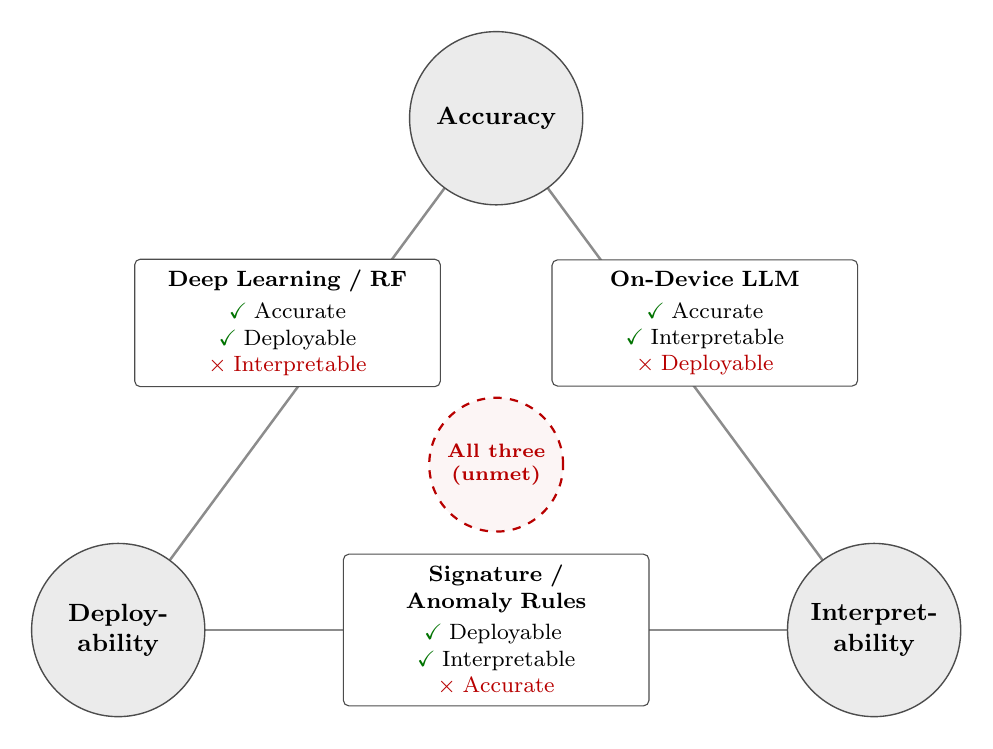
\begin{tikzpicture}[
    font=\footnotesize,
    demand/.style={
        circle, draw=black!70, fill=black!8, line width=0.5pt,
        align=center, minimum size=22mm, inner sep=1pt,
        font=\small\bfseries
    },
    approach/.style={
        draw=black!70, rounded corners=2pt, fill=white,
        align=center, inner sep=4pt, text width=36mm, font=\footnotesize
    },
    edge/.style={draw=black!45, line width=0.9pt},
    unmet/.style={
        circle, draw=bad, dashed, line width=0.8pt, fill=bad!4,
        align=center, minimum size=17mm, font=\scriptsize\bfseries, text=bad
    }
]

% ---- Tight bounding box around the content (no frame, no padding) ----
\useasboundingbox (-5.95,-3.35) rectangle (5.95,5.45);

% ---- Triangle vertices (the three competing demands) ----
\coordinate (A) at (0, 4.3);      % Accuracy
\coordinate (D) at (-4.8,-2.2);   % Deployability
\coordinate (I) at (4.8,-2.2);    % Interpretability

% ---- Triangle edges: each edge is the pair of demands that ONE
%      approach satisfies together ----
\draw[edge] (A) -- (D);
\draw[edge] (D) -- (I);
\draw[edge] (I) -- (A);

% ---- The demands ----
\node[demand] (acc)  at (A) {Accuracy};
\node[demand] (dep)  at (D) {Deploy-\\ability};
\node[demand] (intp) at (I) {Interpret-\\ability};

% ---- The unmet target at the centre ----
\node[unmet] (cpt) at (0,-0.1) {All three\\(unmet)};

% ---- Approaches: each hugs the edge of the two demands it meets,
%      and explicitly fails the third ----
\node[approach] at (-2.65,1.7)
     {\textbf{Deep Learning / RF}\\[2pt]
      \yes{Accurate}\\ \yes{Deployable}\\ \no{Interpretable}};

\node[approach] at (2.65,1.7)
     {\textbf{On-Device LLM}\\[2pt]
      \yes{Accurate}\\ \yes{Interpretable}\\ \no{Deployable}};

\node[approach] at (0,-2.2)
     {\textbf{Signature / Anomaly Rules}\\[2pt]
      \yes{Deployable}\;\; \yes{Interpretable}\\ \no{Accurate}};

\end{tikzpicture}%

\end{document}
